\documentclass{article}
\usepackage{graphicx}
\usepackage{hyperref}
\usepackage{pgfgantt}
\usepackage{amsmath} 
\usepackage{tikz}
\usepackage{pdflscape}
\usetikzlibrary{shapes.geometric, arrows, positioning}

\usepackage{geometry}
\setlength{\parindent}{0pt}
\geometry{margin=3cm}
\title{Project proposal}
\author{Antoine Vitupier, Marcus Hamelink, Antoine Reynaud, Ferdinand Chiu, Ilias Sokolis, Noa Duron}
\date{March 2026}

\begin{document}

\maketitle

\section{Description}

The FaceHugger Robot is a 12-degree-of-freedom legged robot, built to mimic the posture and movement of a four-legged mammal. With four legs each driven by three servo motors, it can shift its weight, adjust its stance, and walk in any direction while keeping its body level and stable. \\

Movement is governed by an 80/20 hybrid model. Eighty percent of the motion comes from hardcoded elliptical foot trajectories that produce a fluid trot gait, giving the robot full 360-degree translation: forward, backward, and lateral strafing in any direction. The remaining twenty percent is a real-time stabilisation layer driven by the IMU. A PID controller reads the current pitch and roll and computes a corrective vertical offset
$\Delta z$ that is applied to all four foot targets simultaneously:
\[
  z_{\mathrm{actual}} = z_{\mathrm{gait}} + \Delta z_{\mathrm{PID}}
\]
This keeps the chassis level over uneven terrain without the gait engine needing any knowledge of the floor geometry. \\

Underlying both layers is an analytical Inverse Kinematics solver. Every foot target is expressed in a global body frame centred on the robot's centre of mass, so a single body-tilt correction automatically propagates to all four legs at once. This is what
gives the robot its characteristic organic appearance: the body floats steadily above shifting feet rather than moving rigidly as one piece. \\

Beyond standard locomotion, the robot supports a signature maneuver: a self-righting wall-flip. When the front ToF sensor detects a wall at close range, the robot can execute a pre-timed open-loop thrust sequence to push off the surface, rotate in the air, and land upright. The IMU monitors the fall and re-engages normal operation automatically once the robot is stable. \\

\subsection*{Primary Objectives}

\begin{enumerate}
  \item \textbf{Stand and self-support.} The robot maintains a stable stance under its own weight with all servos holding position.
  \item \textbf{Teleoperated walking.} A user controls the robot in real time from a smartphone joystick, going forward, backward, lateral, and turning, using the hybrid 80/20 trot gait described above.
  \item \textbf{Command API.} All motion primitives are accessible via a documented WebSocket/JSON interface, enabling programmatic control from any networked device.
\end{enumerate}

\subsection*{Extensions}

\textbf{Bluetooth Person-Following.} A Bluetooth beacon worn by the operator (e.g.\ a second ESP32) lets the robot estimate the bearer's relative direction from RSSI measurements. The robot turns autonomously to track the beacon without requiring a camera or computer vision. \\

\textbf{Self-Righting Wall-Flip.} When the front-facing ToF sensor detects a wall within a threshold distance and the operator issues the \texttt{"flip"} command, the FSM enters the \textsc{action} state, PID stabilisation is suspended, and Core~0 executes a pre-timed
open-loop burst of maximum-torque PWM signals to push the robot off the wall. The IMU monitors orientation and re-engages normal operation once tilt returns below
10\textdegree{}.

% ============================================================

\subsection{Hardware}

The hardware architecture is carefully designed to meet the project’s requirements, particularly the high current demand, which can reach up to \textbf{24A} if all servos operate simultaneously at max current (which is highly unlikely). In the beginning we thought of implementing a distributed power architecture where one DC DC step down buck converter would be used in series with one PCA 9685 PWM multiplexer in each pair of legs to split the current between two pair of legs (12A max each for each pair of legs) and another DC DC step down buck converter to get a 5V output voltage for the micro controller and sensors. 

\vspace{0.5cm}
After talking with the professor and the T.As we deemed that this was unnecessary (as the servos will never operate at max current simultaneously) so we proceeded to go with one PCA 9685 PWM multiplexer directly getting power from the battery (even if the servos are rated to work in the range of 5V-7.2V the professor told us that it will likely be ok to operate it like that) as well as DC DC buck converter to step down the voltage for the microcontroller and sensors.

\subsubsection{Leg movement}
Since we decided to have 3 joints on each leg, we needed to have a total of 12 powerful servos. After carefully reading other projects similar to ours in the past and talking with our T.A. we concluded that the classic SG90 servos do not confortably supply enough torque.

\vspace{0.5cm}
We proceeded with the \textbf{DSS 15Kg*cm 270°} servos because of their rotation versatility, light weight (70g) and powerful torque. Even if they require a lot of current, our battery will be able to comfortably supply it.

\vspace{0.5cm}

Those servos will receive their signals via a PCA 9685 PWM multiplexer and their power directly from the battery connected to the Vin pin of the PCA9685 PWM multiplexer.

\vspace{0.5cm}
The only problem we can think about with this is that when the battery is fully charged (around 8V) it surpasses the maximum recommended operating voltage of the servos, but the professor told us it should not be a problem, if it is we will just use a DC-DC buck converter that supports large currents (around 10-15A) to step down the voltage of the battery.

\subsubsection{Central Processing Unit}

For the brain of our robot, we chose an \textbf{ESP32 Devkit V1 Wifi/Bluetooth Dual Core micro controller}. The dual core setup enables us to divide our software architecture in two parts (see below): core 1 handles the \textbf{JSON parsing of the packets} coming from our remote control app while core 2 handles the \textbf{nervous system} of the robot (inverse kinematics engine). The \textbf{Wifi/Bluetooth} functionality enables us to \textbf{remotely control} the robot via our Command API and the numerous ports enable us to equip our robot with the sensors required via an \textbf{I2C multiplexer}.

\subsubsection{Sensors}

For the senses of the FaceHugger, we chose to give it an \textbf{accelerometer + gyroscope} sensor which is essential to understanding the robot's current orientation and speed in order to be able to maneuver more complex terrains such as stairs while keeping the equilibrium. We also decided to equip it with 5 time of flight distance sensors (\textbf{VL53L0X (ToF) I2C Laser Distance Sensor}) for the front, left, right, back and bottom part of robot, in order to be able to detect its surroundings if we want to extend it to be more autonomous. The sensors will get power via the 3.3V voltage output pin of the ESP32 microcontroller.

\vspace{0.5cm}
We also decided to add a small \textbf{SBC-OLED screen} in order to give a "face" to our robot.

\subsubsection{Power \& Power Management}

For the heartbeat of our robot we chose a \textbf{2S 1300 mAh 30C (39A max) LiPo battery} connected in series with a battery protection module as well as an on/off switch to switch off/on the robot to which we will connect 1 buck converter and one PCA 9685 PWM multiplexer in parallel:

\begin{itemize}

\item{\textbf{LM2596 DC-DC Step-Down Converter Module with Display} to connect to the ESP32 controller (stepped down to 5V) that will supply power both to the micro controller and the sensors}

\item{\textbf{PCA 9685 PWM multiplexer} to connect the servos that will get power directly from the battery}
\end{itemize}
%\item{One \textbf{300W 20A DC-DC Step-down buck converter} which will supply power for the first pair of legs over a \textbf{PCA 9685 PWM multiplexer} (around 7V). This will control the first pair of legs.}

%\item{Another \textbf{300W 20A DC-DC Step-down buck converter} with a \textbf{PCA 9685 PWM Multiplexer} in exactly the same configuration, controlling the other pair of legs.}









\subsection{Software}
The software architecture is designed to manage the high computational demands of 12-DOF Inverse Kinematics (IK) and real-time stability by leveraging the ESP32’s dual-core processor. We utilize a FreeRTOS multitasking environment to ensure that time-critical motor movements are never interrupted by network latency or sensor polling.

\subsubsection{Dual-Core Execution Model}
To maintain smooth and responsive movement, the software is partitioned into two primary execution loops:
\begin{itemize}
    \item \textbf{Core 0 (Nervous System):} Dedicated to the high-frequency Kinematics loop ($50\text{Hz}$--$100\text{Hz}$). This core calculates joint angles and updates the PCA9685 PWM multiplexer.
    \item \textbf{Core 1 (Brain):} Manages high-level logic, including WiFi/WebSocket communication, JSON packet parsing from the remote controller, and sensor fusion from the IMU and ToF sensors.
\end{itemize}

\subsubsection{Inverse Kinematics (IK) Implementation}
Inverse Kinematics is the mathematical process of calculating required joint angles ($\theta_1, \theta_2, \theta_3$) to reach a specific coordinate $(x, y, z)$. This is fundamental for achieving smooth and controlled movement without manually programming every servo rotation.
\begin{itemize}
    \item \textbf{Geometric Modeling:} Using measurements from our CAD design, we apply trigonometric identities to map the workspace of each leg.
    \item \textbf{Gait Integration:} IK allows us to define "steps" as parametric elliptical paths, enabling the robot to walk forward, backward, or laterally.
    \item \textbf{Stability:} By decoupling foot position from servo angles, we can dynamically shift the center of mass to maintain balance when standing on fewer than four legs.
\end{itemize}

\subsubsection{Control Philosophy: The 80/20 Hybrid Model}
Stability is the primary challenge for our quadruped. We implement a hybrid control strategy to balance reliability with environmental reactivity:
\begin{itemize}
    \item \textbf{Open-Loop Trajectories (80\%):} The robot follows pre-calculated elliptical paths for forward, backward, and lateral (strafing) gaits.
    \item \textbf{Reactive Stabilization (20\%):} A PID Controller uses real-time data from the MPU6050 IMU to calculate body-tilt offsets. These offsets are added to the leg coordinates to keep the chassis level on uneven terrain.
\end{itemize}

\subsubsection{Finite State Machine (FSM)}
The robot's behavior is governed by a State Machine to ensure safe transitions between maneuvers:
\begin{itemize}
    \item \textbf{IDLE:} Active balancing is enabled; the robot utilizes the PID loop to resist external tilting forces.
    \item \textbf{WALK:} The gait engine is active, merging hardcoded steps with dynamic PID leveling.
    \item \textbf{ACTION:} Specialized sequences, such as the Wall-Flip, are triggered. The ToF sensors verify wall proximity before inhibiting stabilization to allow high-torque rotation.
    \item \textbf{FAILSAFE:} A safety interrupt cuts power to the servos if the battery voltage drops below a certain threshold or if a fall is detected. Precise details
\end{itemize}


\subsubsection{Code Architecture Flow}
The interaction between the user, the environment, and the dual-core execution
is visualized in the following logic flow:

\begin{center}
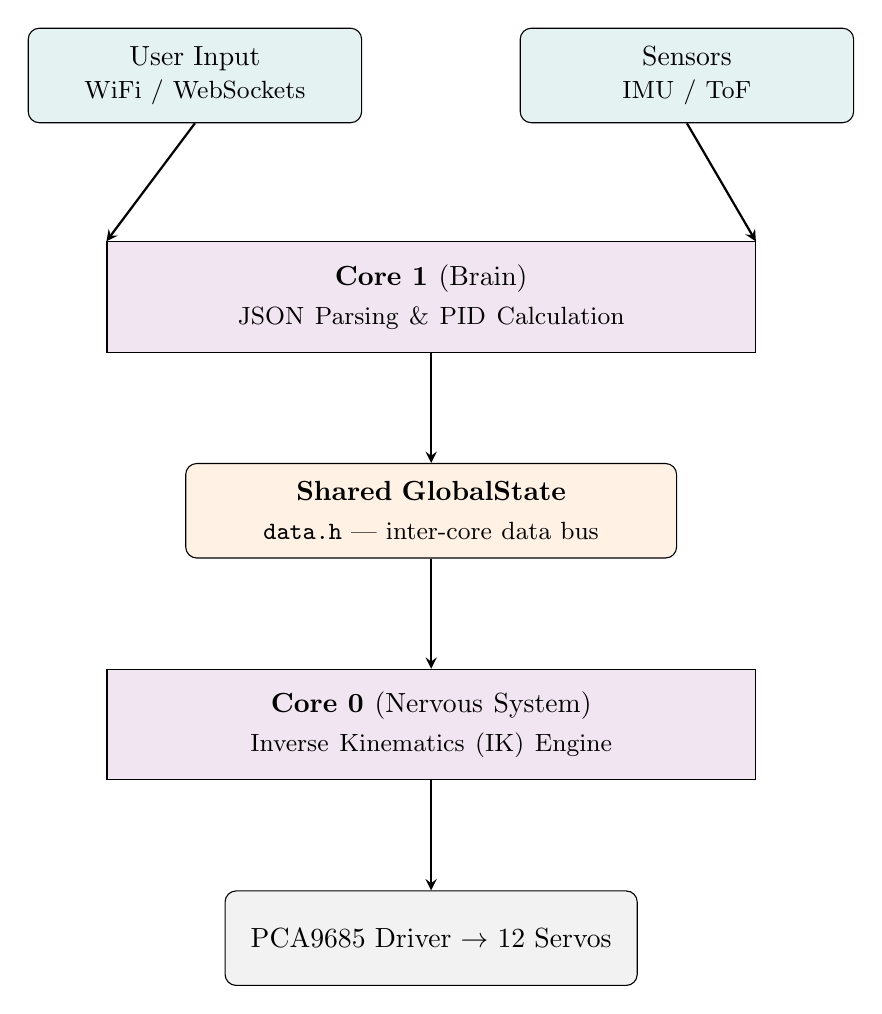
\begin{tikzpicture}[
    node distance=1.5cm,
    block/.style={
        rectangle, draw, fill=teal!10, text width=4cm,
        text centered, rounded corners, minimum height=1.2cm
    },
    core/.style={
        rectangle, draw, fill=violet!10, text width=8cm,
        text centered, minimum height=1.4cm, font=\bfseries
    },
    shared/.style={
        rectangle, draw, fill=orange!10, text width=6cm,
        text centered, rounded corners, minimum height=1.2cm
    },
    output/.style={
        rectangle, draw, fill=gray!10, text width=5cm,
        text centered, rounded corners, minimum height=1.2cm
    },
    arrow/.style={thick, ->, >=stealth}
]

%% Input layer
\node (input)   [block] {User Input \\ \small WiFi / WebSockets};
\node (sensors) [block, right=2cm of input] {Sensors \\ \small IMU / ToF};

%% Core 1
\node (core1) [core, below=1.5cm of input, xshift=3cm]
    {Core 1 \textnormal{(Brain)} \\[2pt]
     \normalfont\small JSON Parsing \& PID Calculation};

%% Shared state
\node (state) [shared, below=1.4cm of core1]
    {\textbf{Shared GlobalState} \\[2pt]
     \normalfont\small \texttt{data.h} — inter-core data bus};

%% Core 0
\node (core0) [core, below=1.4cm of state]
    {Core 0 \textnormal{(Nervous System)} \\[2pt]
     \normalfont\small Inverse Kinematics (IK) Engine};

%% Output
\node (out) [output, below=1.4cm of core0]
    {PCA9685 Driver $\rightarrow$ 12 Servos};

%% Arrows
\draw [arrow] (input.south)   -- (core1.north west);
\draw [arrow] (sensors.south) -- (core1.north east);
\draw [arrow] (core1.south)   -- (state.north);
\draw [arrow] (state.south)   -- (core0.north);
\draw [arrow] (core0.south)   -- (out.north);

\end{tikzpicture}
\end{center}

This separation ensures that the \textbf{Nervous System} maintains a deterministic refresh rate for the servos, while the \textbf{Brain} handles asynchronous tasks like network requests and sensor filtering without causing physical lag in the robot's movement.

\subsubsection{Repository Partitioning Scheme}
The following directory tree illustrates the modular separation of the robot's control systems:

\begin{center}
\resizebox{\textwidth}{!}{%
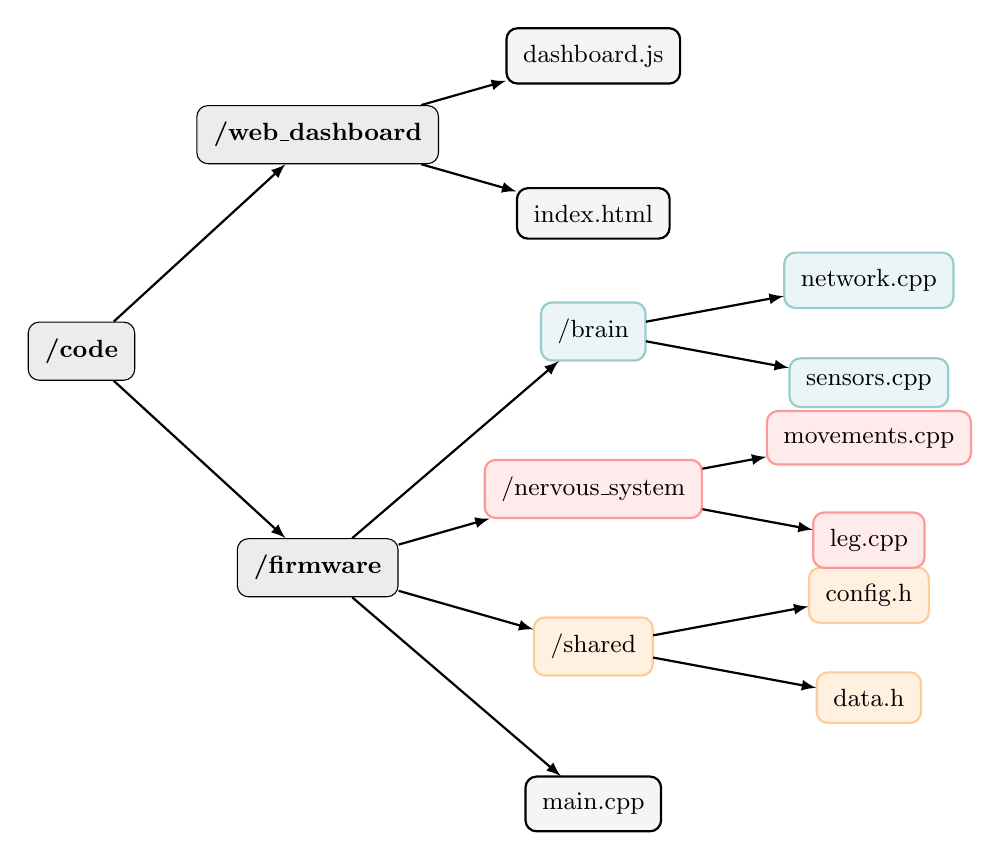
\begin{tikzpicture}[
    grow=right,
    level 1/.style={sibling distance=5.5cm,  level distance=3cm},
    level 2/.style={sibling distance=2cm,    level distance=3.5cm},
    level 3/.style={sibling distance=1.3cm,  level distance=3.5cm},
    edge from parent/.style={draw, -latex, thick},
    every node/.style={
        rectangle, draw, rounded corners,
        fill=gray!8, inner sep=6pt, font=\small
    },
    dir/.style     ={fill=gray!15, font=\small\bfseries},
    nervous/.style ={fill=red!8,    draw=red!40},
    brain/.style   ={fill=teal!8,   draw=teal!40},
    shared/.style  ={fill=orange!12, draw=orange!40}
]
\node [dir] {/code}
    child { node [dir] {/firmware}
        child { node {main.cpp} }
        child { node [shared] {/shared}
            child { node [shared] {data.h} }
            child { node [shared] {config.h} }
        }
        child { node [nervous] {/nervous\_system}
            child { node [nervous] {leg.cpp} }
            child { node [nervous] {movements.cpp} }
        }
        child { node [brain] {/brain}
            child { node [brain] {sensors.cpp} }
            child { node [brain] {network.cpp} }
        }
    }
    child { node [dir] {/web\_dashboard}
        child { node {index.html} }
        child { node {dashboard.js} }
    };
\end{tikzpicture}%
}
\end{center}

This is how we plan to organize our code for the moment, clearly separating the web dashboard part from the actual implementation of the movement of the quadruped .

\subsection{Physical Structure}

\section{CAD Design}
% ============================================================
% SECTION 2: CAD DESIGN
\begin{verbatim}
Manual (8.1, 8.5.2): Complete technical drawings of all structural
and mechanical parts, produced in Fusion 360. Must show dimensions
so staff can verify parts in the BOM are appropriate.
Formal CAD drawings required — no hand-drawn sketches.
CAD is a living document, updated throughout the semester.

For Ferdinand
\end{verbatim}
% ============================================================
\subsection{Technical drawings}
\subsection{Circuit diagram}
% ============================================================

\section{Risk Assessment}

\begin{enumerate}
    \item \textbf{Weight, leg lever-arms, and servo strength (torque margin)} \\
    \textit{What could go wrong:} BeetleBot identified weight/servo strength as a main project risk and later reported that early leg designs were too long/heavy, making it hard or impossible to stand/walk without overloading servos; even after optimization, servos still struggled. For our \textbf{quadruped}, this risk is higher because each leg carries a larger fraction of the total load and there is less redundancy than a hexapod. If torque margin is insufficient, we will fail to achieve a stable stand and any walking demo. \\
    \textit{Mitigation (prototype + when):} By \textbf{Week 6}, prototype a \textbf{single-leg + hip load test} (or 2-leg front module) to validate stall/hold performance at the worst joint angles. We will explicitly design for short lever arms (legs closer under the body), keep heavy components low/central, and reduce printed mass (cutouts, low infill where safe). If results are marginal, we will (i) reduce leg length/stance height and (ii) upgrade only the most loaded joints to higher-torque servos before procurement is locked.

    \item \textbf{LiPo power delivery and brownouts during peak servo load} \\
    \textit{What could go wrong:} BeetleBot flagged LiPo + regulation as risky: many servos moving together can cause voltage drops, resets, and servo glitches. Our system similarly uses a single battery with a 5V rail feeding many servos (via PCA9685) plus the ESP32; sudden current peaks (startup/stall) can reset the ESP32 or cause unstable behavior that appears as a software issue. \\
    \textit{Mitigation (prototype + when):} By \textbf{Week 6--7}, bench-test the full power chain (LiPo $\rightarrow$ buck $\rightarrow$ servo rail + logic rail) with worst-case motion patterns. Use thick wiring for the servo rail, star grounding, and bulk capacitance near the servo supply. Implement software-side current shaping: avoid commanding all joints to step simultaneously (ramping/interpolation) and enforce conservative acceleration/step height. If necessary, split rails (separate regulator for ESP32) or keep an optional second battery plan.

    \item \textbf{Servo coordination, timing, and smoothness (control loop reliability)} \\
    \textit{What could go wrong:} BeetleBot explicitly noted that coordinating many servos is challenging (timing, synchronization, responsiveness). For our quadruped, control jitter or blocking code will directly translate into instability (falls) and will slow tuning significantly. \\
    \textit{Mitigation (prototype + when):} Use a fixed-rate motion update loop on ESP32 (target $50$--$100$ Hz) and keep time-critical motor updates isolated from network and sensor tasks (FreeRTOS priorities / dual-core split). Start with \textbf{basic primitives} (stand, shift weight, lift one foot) before full gaits, and use interpolation/ramping for smooth trajectories.

    \item \textbf{IK implementation sensitivity to real-world measurements and calibration} \\
    \textit{What could go wrong:} BeetleBot’s proposal and README both show IK is measurement-sensitive: small differences in link lengths/servo positions can produce inaccurate motion, and tuning can become time-consuming late in the project. If our CAD measurements do not match the built robot, gaits will drift, legs may bind, and stability control will be unreliable. \\
    \textit{Mitigation (prototype + when):} By \textbf{Week 7--8}, implement a calibration mode: center servos, store per-servo offsets, enforce joint limits, and verify foot positions on a test stand. Measure real link lengths and update IK constants accordingly. Maintain a fallback “hardcoded stance / crawl” mode (like BeetleBot’s compromise approach) so integration/testing can proceed even if IK is still being refined.

    \item \textbf{Gait stability for a quadruped (risk of spending too long on dynamic gaits)} \\
    \textit{What could go wrong:} BeetleBot emphasized stability and balance (center of mass must remain within support polygon) and planned both static and dynamic stability work. A quadruped has tighter stability constraints than a hexapod; attempting dynamic gaits (trot/dance) too early can lead to repeated failures and jeopardize the demo. \\
    \textit{Mitigation (prototype + when):} By \textbf{Week 8--9}, target a robust \textbf{static crawl} (3 feet down) and stable pose transitions (sit/stand). Only after this baseline works will we attempt faster gaits as \textbf{optional extensions}. PID-based leveling (IMU) will be introduced progressively: first validate open-loop crawl, then add stabilization and re-tune step sizes.

    \item \textbf{Remote control over WiFi/WebSocket: integration complexity and coupling to motion control} \\
    \textit{What could go wrong:} BeetleBot identified remote control as an additional complexity layer and noted that WiFi/Web APIs require background knowledge; tight coupling between comms and walking logic increases debugging difficulty. For our system, network latency or parsing delays could interfere with control timing if not isolated. \\
    \textit{Mitigation (prototype + when):} Keep communication logic modular and separate from motion control (queue commands from “brain” task to “nervous system” task). Define a minimal protocol (small JSON messages is acceptable if rate-limited). Validate the web interface early on a bench setup (ESP32 + PCA9685 + 1--2 servos). Maintain a serial “manual override” fallback for debugging if WiFi issues appear.

\item \textbf{Demount/remount difficulty (maintenance and iteration speed)} \\
\textit{What could go wrong:} Based on prior legged-robot experience (e.g., BeetleBot’s emphasis on complex cable management and frequent hardware access), a major schedule risk is having a design that is hard to open, service, or reassemble. If servos, the PCA9685, sensors, or the ESP32 are not easily accessible, every failure (servo replacement, wire debugging, re-printing one part, re-routing cables) becomes a long operation. This slows down iteration, increases the chance of wiring mistakes after reassembly, and can block integration/testing late in the project. \\
\textit{Mitigation (prototype + when):} By \textbf{Week 6--7}, enforce a \textbf{serviceable mechanical/electrical design}:
(i) split the chassis into modules (e.g., leg modules + electronics bay),
(ii) use a lid/cover with a small number of standard fasteners and clear access to the PCA9685 and power chain,
(iii) add strain relief and tie points so cable bundles keep their shape during opening/closing,
(iv) label connectors and define a fixed pin map,
(v) time a “maintenance drill” (open body, replace one servo, close body) and iterate CAD until it can be done quickly and repeatably.    
\end{enumerate}



\section{Bill of Materials}
% ============================================================
% SECTION 4: BILL OF MATERIALS
% ============================================================

For the bill of materials we will need (see Table 1):

\begin{table}[h]
\centering
\begin{tabular}{|p{4cm}|l|l|r|}
\hline
\textbf{Item} & \textbf{Qty} & \textbf{Source / Link} & \textbf{Price (CHF)} \\
\hline
ESP32 Devkit V1 Wifi/Bluetooth Dual core & 1 & \href{https://www.conrad.ch/fr/p/carte-de-developpement-joy-it-sbc-nodemcu-esp32-node-mcu-esp32-modul-1656367.html?insert=UP&utm_source=google-shopping-de&utm_medium=search&utm_campaign=shopping-online-de&utm_content=shopping-ad_cpc&WT.srch=1&ef_id=CjwKCAjwyYPOBhBxEiwAgpT8P118jEa1ibbm1lb82e_rh13doZgsRWLhNMrAkNIhP5DfltGE-hYAXhoCzpUQAvD_BwE:G:s&utm_source=google&utm_medium=cpc&utm_campaign=PMax%3A%20Smart%20Shopping%20Kampagne&utm_id=18356446076&gad_source=1&gad_campaignid=17418395455&gbraid=0AAAAADzhVTvb4LkDAI55YARL_6ZQ3Kq5d&gclid=CjwKCAjwyYPOBhBxEiwAgpT8P118jEa1ibbm1lb82e_rh13doZgsRWLhNMrAkNIhP5DfltGE-hYAXhoCzpUQAvD_BwE}{Link to buy} & 8\\
\hline
PCA9685 PWM Multiplexer & 1 & \href{https://www.conrad.ch/de/p/iduino-me234-motortreiber-1-st-passend-fuer-entwicklungskits-arduino-2315243.html?insert=UP&utm_source=google-shopping-de&utm_medium=search&utm_campaign=shopping-online-de&utm_content=shopping-ad_cpc&WT.srch=1&ef_id=CjwKCAjwyYPOBhBxEiwAgpT8Pwr1OnDVIuYLSpyQh8hTdGKrH1Eavqnk8U7DHi8e3p-7Ys8PuAcHJRoCMzcQAvD_BwE:G:s&utm_source=google&utm_medium=cpc&utm_campaign=PMax%3A%20Smart%20Shopping%20Kampagne&utm_id=18356446076&gad_source=1&gad_campaignid=17418395455&gbraid=0AAAAADzhVTvb4LkDAI55YARL_6ZQ3Kq5d&gclid=CjwKCAjwyYPOBhBxEiwAgpT8Pwr1OnDVIuYLSpyQh8hTdGKrH1Eavqnk8U7DHi8e3p-7Ys8PuAcHJRoCMzcQAvD_BwE}{Link to buy} & 11\\
\hline
15Kg/cm 270° Servo DSS-M15S with Metal Gear & 12 & \href{https://www.mouser.ch/ProductDetail/DFRobot/SER0038?qs=lqAf%2FiVYw9jKMX2bo90oYQ%3D%3D}{Link to buy} & 145\\
\hline
Li-Po 2S 7,4V 30C 1.300 mAh, contact JST-RCY (BEC) & 1 & \href{https://www.galaxus.ch/fr/s5/product/hacker-lipo-pack-tf-eco-x-1300mah-3s-mtag-1110-v-1300-mah-batterie-rc-12684610}{Link to buy} & 20 \\
\hline
IMU MPU6050 Accelerometer + Gyroscope & 1 & \href{https://www.galaxus.ch/fr/s1/product/purecrea-mpu-6050-accelerometre-3-axes-avec-gyroscope-carte-de-developpement-kit-36359715?offertype=marketplace&offerid=8244233&utm_source=google&utm_medium=cpc&utm_campaign=PMax%3A+PROD_CH_SSC_Cluster_2%28C%29&campaignid=20399813757&adtype=pla&adgroupid=&adid=&dgCidg=CjwKCAjwyYPOBhBxEiwAgpT8P34CuotpLdwayrLMM1MMjXqTSw5O2w66k-yQuVaAeBgs8f846UuUhhoC0_4QAvD_BwE&dgCidg=CjwKCAjwyYPOBhBxEiwAgpT8P34CuotpLdwayrLMM1MMjXqTSw5O2w66k-yQuVaAeBgs8f846UuUhhoC0_4QAvD_BwE&gclsrc=aw.ds&gad_source=1&gad_campaignid=19973636350&gbraid=0AAAAADmCc4M3D0rGPgLdZCT94mDOGgxSi&gclid=CjwKCAjwyYPOBhBxEiwAgpT8P34CuotpLdwayrLMM1MMjXqTSw5O2w66k-yQuVaAeBgs8f846UuUhhoC0_4QAvD_BwE}{Link to buy} & 13 \\
\hline
VL53L0X (ToF) I2C Laser Distance Sensor & 5 & \href{https://www.mouser.ch/ProductDetail/DFRobot/SEN0245?qs=vdi0iO8H4N2%252ByTl%252BC%252Bk6RA%3D%3D}{Link to buy} & 30 \\
\hline
%300W 20A DC-DC Step-down Module, Constant Voltage and Constant Current Adjustable Vehicle Charging Module & 2 & \href{https://www.joom.com/en/products/67037cacc862c801406e069c?currency=CHF&utm_productid=67037cacc862c801406e069c&utm_feed=web&utm_hash=ea390b582ec73a07e0936cb0dc64965b&variant_id=67037cacc862c848406e069e&gsAttrs=eyJyZWdpb24iOiJDSCIsICJzcGVjaWFsUHJpY2VVc2VkIjpmYWxzZX0g&exp_price=MTMuMSAg&country=CH&utm_audienceid=advertising_web_impact_2d&click_id=ydnRCJx3yxyZRkB1PQUgoReHUkuwMsQe0TXsQQ0&sharedid=&utm_medium=partners&utm_source=impact&utm_campaign=2414876&irgwc=1&afsrc=1}{Link to buy} & 25 \\
%\hline

LM2596 DC-DC Step-Down Converter Module with Display to connect with ESP32 controller + sensors & 1 & \href{https://www.bastelgarage.ch/components/power-supplies-electricity/dc-dc-converter-step-down/lm2596-dc-dc-step-down-converter-module-with-display}{Link to buy} & 10 \\
\hline
Female XT60 connector & 2 & \href{https://www.conrad.ch/fr/p/reely-re-6702318-prise-femelle-pour-batterie-xt60-dore-e-1-pc-s-2234106.html}{Link to buy} & 2 \\
\hline
Male XT60 connector & 2 & \href{https://www.bastelgarage.ch/components/power-supplies-electricity/dc-dc-converter-step-down/lm2596-dc-dc-step-down-converter-module-with-display}{Link to buy} & 2 \\
\hline
ON/OFF switch & 1 & \href{https://www.mouser.ch/ProductDetail/Bulgin/C7510T110R?qs=yc9RBI4tIAKVWqYUySD3pw%3D%3D}{Link to buy} & 1 \\
\hline
I2C multiplexer & 1 & \href{https://www.mouser.ch/ProductDetail/Adafruit/2717?qs=FXKxjuMTmBk%252BXQsxVhda7A%3D%3D}{Link to buy} & 5 \\
\hline
Battery protection module for lipo 2S 1300 mAh 30C (39A) & 1 & \href{}{Link to buy} & 10 \\
\hline
XT60 Charging cable & 1 & \href{https://www.swaytronic.ch/en/SWAYTRONIC-charging-cable-XT60}{Link to buy} & 5 \\
\hline
SBC-OLED01V2 128x64 pixels I2C screen & 1 & \href{https://www.galaxus.ch/fr/s1/product/joy-it-sbc-oled01v2-module-daffichage-24-cm-096-pouce-128-x-64-pixels-carte-de-developpement-kit-49727962?offertype=marketplace&offerid=8902998&utm_source=google&utm_medium=cpc&utm_campaign=PMax%3A+PROD_CH_SSC_Cluster_1%28C%29&campaignid=20421516236&adtype=pla&adgroupid=&adid=&dgCidg=CjwKCAjwspPOBhB9EiwATFbi5I3IFC64J6Kvxk-0IQ-IzSVstY82pjj-WPzB2ywz78h0xKiLJKn2GhoCYfoQAvD_BwE&dgCidg=CjwKCAjwspPOBhB9EiwATFbi5I3IFC64J6Kvxk-0IQ-IzSVstY82pjj-WPzB2ywz78h0xKiLJKn2GhoCYfoQAvD_BwE&gclsrc=aw.ds&gad_source=1&gad_campaignid=19973634409&gbraid=0AAAAADmCc4OuDq76iQruiz45zypmbMG5e&gclid=CjwKCAjwspPOBhB9EiwATFbi5I3IFC64J6Kvxk-0IQ-IzSVstY82pjj-WPzB2ywz78h0xKiLJKn2GhoCYfoQAvD_BwE}{Link to buy} & 10 \\
\hline
\multicolumn{3}{|r|}{\textbf{Total}} & \textbf{272} \\
\hline
\end{tabular}
\caption{Bill of Materials}
\end{table}


\section{Work Breakdown}
% ============================================================
% SECTION 5: WORK BREAKDOWN
% ============================================================
\newpage
\begin{landscape}
\begin{figure}[]
\centering
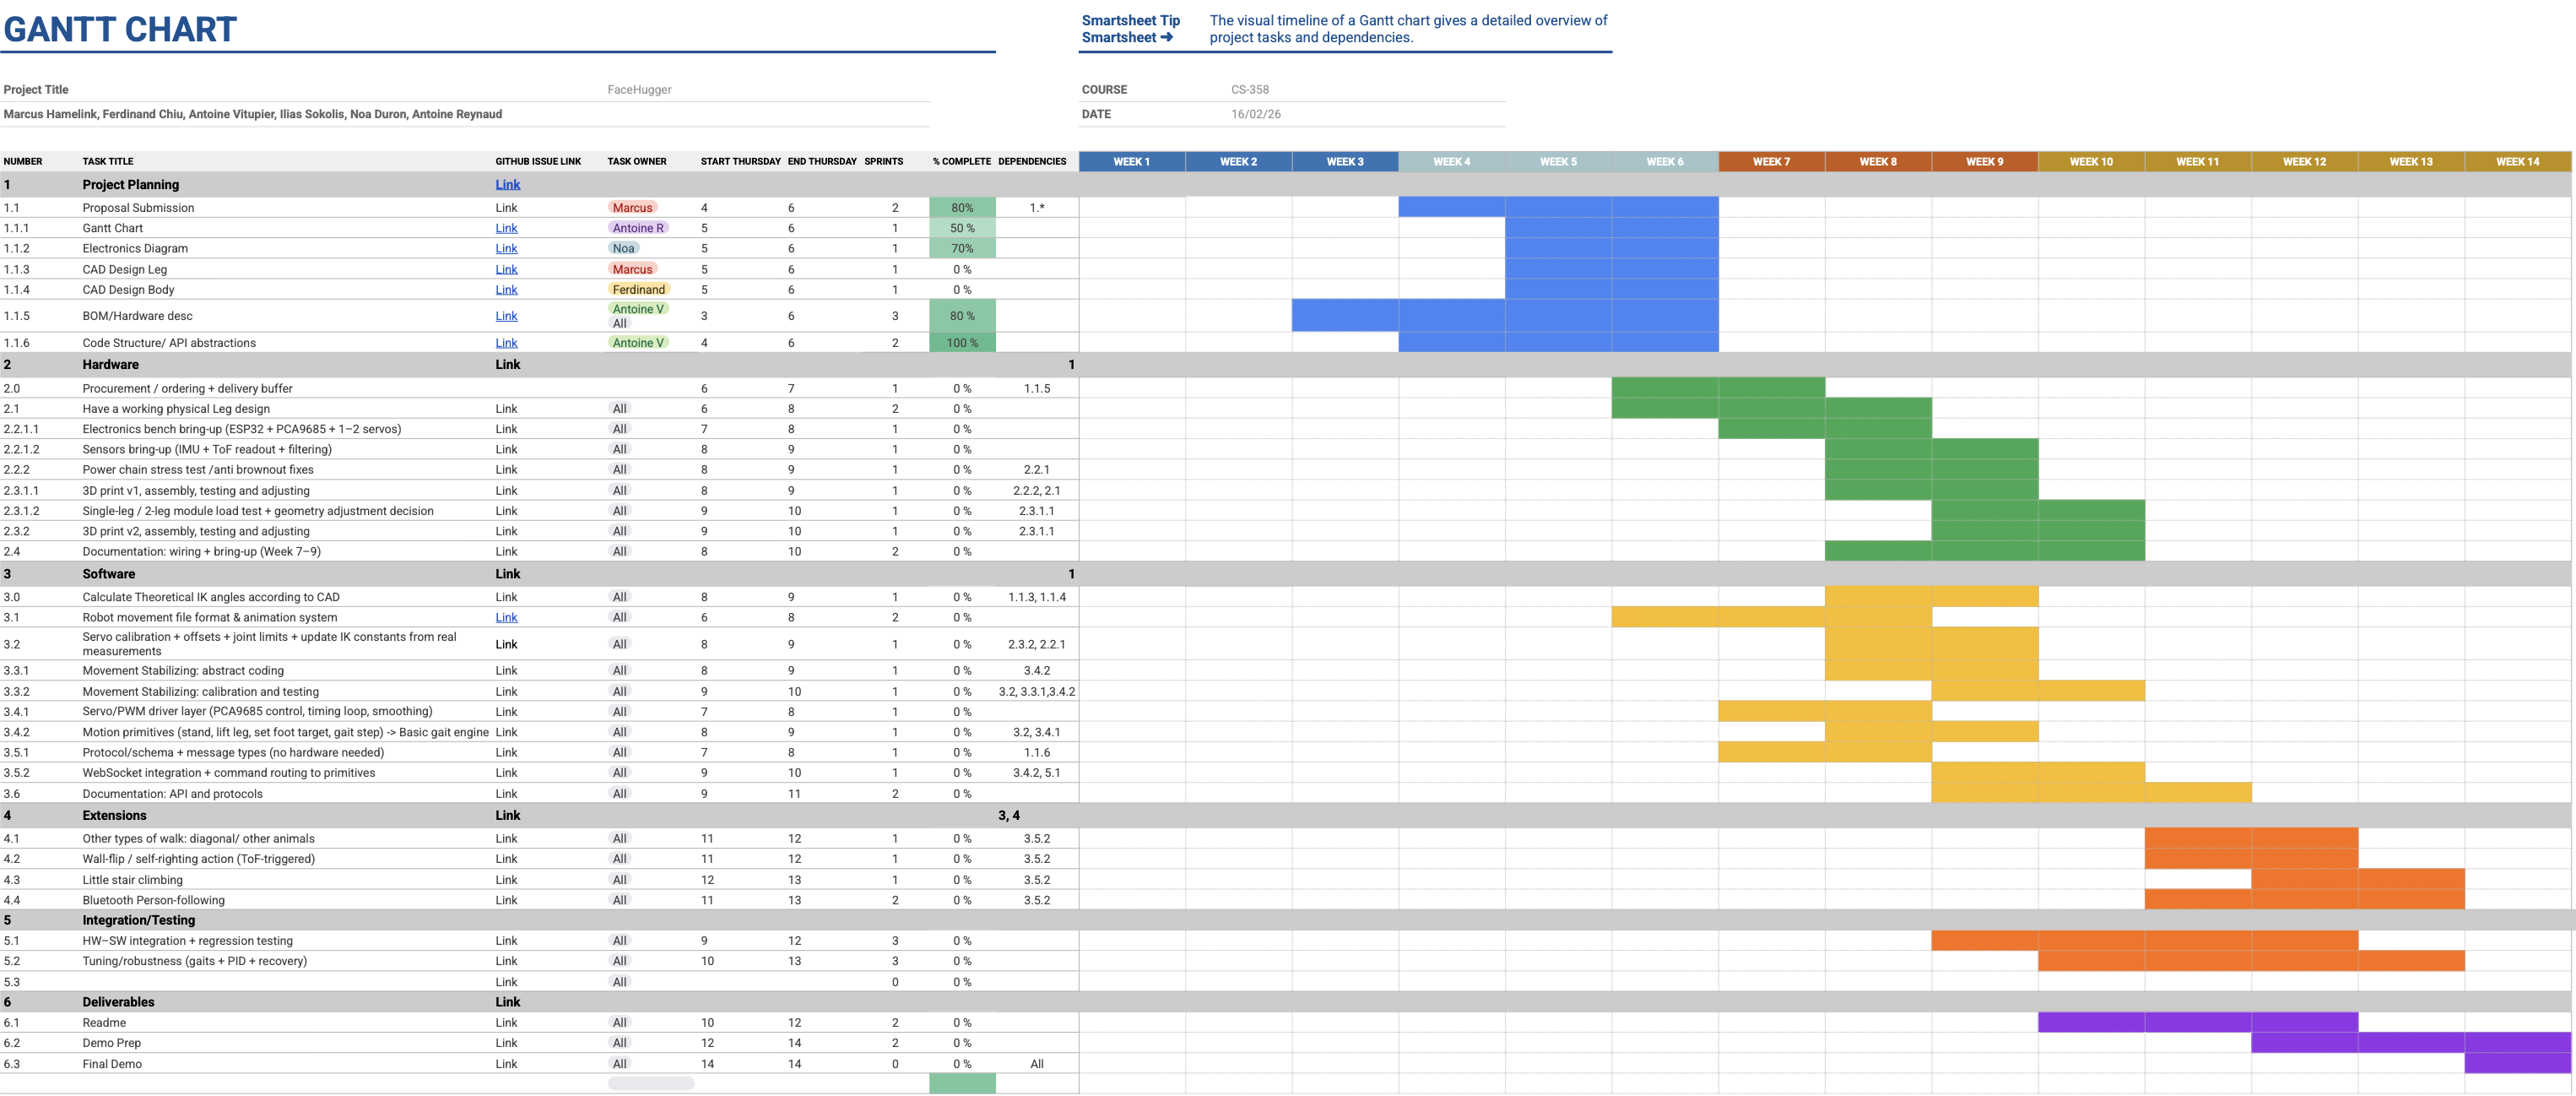
\includegraphics[ scale=0.45]{gantt_chart.png}
\end{figure}
\end{landscape}
\newpage
\section{Future of the FaceHugger}
The current version of the FaceHugger serves as a high-performance 12-DOF baseline. Future iterations could focus on transitioning the robot from a teleoperated machine to an autonomous, environment-aware agent:

\begin{itemize}
    \item \textbf{Vision-Based Spatial Awareness:} By integrating an \textbf{ESP32-CAM} or a small \textbf{LiDAR} module, the robot could move beyond simple ToF distance measurements. This would allow for SLAM (Simultaneous Localization and Mapping), enabling the FaceHugger to navigate complex indoor environments and autonomously plan paths around obstacles.
    
    \item \textbf{Transition to Full Dynamic Stability:} As the gait engine matures, shift the 80/20 hybrid model toward a more reactive model. By utilizing high-frequency IMU feedback and ground-contact sensors in the feet, the robot could achieve "blind" stabilization—navigating stairs or slippery surfaces where hardcoded elliptical paths are insufficient.
    
    \item \textbf{Terrain Adaptation and Obstacle Scaling:} With the 270\textdegree{} range of the \textbf{DSM 15-270} servos, the FaceHugger has the mechanical potential for extreme reach. Future software updates would include a "High-Step" mode, where the robot uses its ToF sensors to measure the height of a ledge and dynamically recalculates its Inverse Kinematics to mount obstacles up to 10cm in height.
    
    \item \textbf{Edge-AI for Gesture Control:} Utilizing the dual-core capability further, Core 1 could run lightweight Machine Learning models to recognize hand gestures or follow a specific person without the need for a Bluetooth beacon, making the interaction more organic.
\end{itemize}

\section{References and Inspirations}

\textbf{BeetleBot — EPFL CS-358 (2025 Hexapod)} \\
\textit{Source:} \url{https://github.com/epfl-cs358/2025sp-beetlebot} \\
\textit{Relevance:} Provided the baseline for the ESP32/PCA9685 wiring topology and highlighted the critical need to upgrade from SG90 to high-torque servos to avoid structural failure. 
\\

\textbf{ResearchGate — Four-Legged 12-Joint Robot CAD Model} 
\textit{Source:} \\
\url{https://www.researchgate.net/figure/fig2_384894431} \\
\textit{Relevance:} Serves as the primary structural blueprint for our 3-DOF leg assembly, specifically guiding the placement of the abduction servos to maximize lateral stability. \\

\textbf{Petoi OpenCat / Bittle (Quadruped)} \\
\textit{Source:} \url{https://github.com/PetoiCamp/OpenCatEsp32} \\
\textit{Relevance:} Validated that a dual-core ESP32 can handle 12-DOF Inverse Kinematics on-chip and served as the primary reference for gait-switching logic (Walk vs. Trot). \\

\textbf{Stanford Pupper (Research Quadruped)} \\
\textit{Source:} \url{https://github.com/stanfordroboticsclub/StanfordQuadruped} \\
\textit{Relevance:} Informed our 80/20 hybrid control philosophy, specifically the use of parametric elliptical trajectories for the swing phase and stance-width calculations. \\

\textbf{Sesame Robot (Expressive Quadruped)} \\
\textit{Source:} \url{https://github.com/dorianborian/sesame-robot} \\
\textit{Relevance:} Inspired the "emotive" extensions of our project, demonstrating how an OLED face can sync with state-machine transitions to indicate robot "mood" or battery status. \\

\textbf{Instructables Spider Robot (Minimal Quadruped)} \\
\textit{Source:} \url{https://www.instructables.com/Spider-Robot-DIY-Quadruped} \\
\textit{Relevance:} Served as a fundamental proof-of-concept for the I2C communication chain and the basic 8-DOF coordinate mapping for 3D-printed quadruped limbs. \\

\end{document}
